%%%%%%%%%%%%%%%%%%%%%%%%%%%%%%%%%%%%%%%%%%%%%%%%%%%%%%%%%%%%%%%%%%%%%%
% Overleaf (WriteLaTeX) Example: Molecular Chemistry Presentation
%
% Source: http://www.overleaf.com
%
% In these slides we show how Overleaf can be used with standard 
% chemistry packages to easily create professional presentations.
% 
% Feel free to distribute this example, but please keep the referral
% to overleaf.com
% 
%%%%%%%%%%%%%%%%%%%%%%%%%%%%%%%%%%%%%%%%%%%%%%%%%%%%%%%%%%%%%%%%%%%%%%

\documentclass{beamer}

\mode<presentation>
{
  \usetheme{Madrid}       % or try default, Darmstadt, Warsaw, ...
  \usecolortheme{default} % or try albatross, beaver, crane, ...
  \usefonttheme{default}    % or try default, structurebold, ...
  \setbeamertemplate{navigation symbols}{}
  \setbeamertemplate{caption}[numbered]
} 

\usepackage[english]{babel}
\usepackage[utf8x]{inputenc}
\usepackage{chemfig}
\usepackage[version=3]{mhchem}

\usepackage{hyperref}
  \hypersetup{colorlinks=true}
  \hypersetup{urlcolor=blue}
  \hypersetup{linkcolor = .}
\usepackage{xcolor}
\usepackage{siunitx}
  \sisetup{separate-uncertainty = true}
\usepackage{physics}
\usepackage[font=small,labelfont=bf]{caption}
\usepackage{subcaption}
\usepackage[en-GB]{datetime2}
\usepackage{feynmp}
\DeclareGraphicsRule{*}{mps}{*}{}

\usepackage{scalerel}
\newcommand{\mylbrace}[2]{\vspace{#2pt}\hspace{6pt}\scaleleftright[\dimexpr5pt+#1\dimexpr0.06pt]{\lbrace}{\rule[\dimexpr2pt-#1\dimexpr0.5pt]{-4pt}{#1pt}}{.}}
\newcommand{\myrbrace}[2]{\vspace{#2pt}\scaleleftright[\dimexpr5pt+#1\dimexpr0.06pt]{.}{\rule[\dimexpr2pt-#1\dimexpr0.5pt]{-4pt}{#1pt}}{\rbrace}\hspace{6pt}}

% Here's where the presentation starts, with the info for the title slide
\title[BESIII Oxford]{BESIII Oxford Group Meeting}
\author{Martin Tat}
\institute{Oxford LHCb}
\date{22nd April 2021}

\titlegraphic{
\includegraphics[width = 5cm, height = 3.8cm]{lhcb.jpg}\hspace{1cm}~%
              
\includegraphics[width = 5cm, height = 3.8cm]{bes3.jpg}}

\begin{document}

\begin{frame}
  \titlepage
\end{frame}

% These three lines create an automatically generated table of contents.
%\begin{frame}{Outline}
%  \tableofcontents
%\end{frame}

\section{Intorduction}
\begin{frame}{Introduction}
  \begin{itemize}
    \setlength\itemsep{2em}
    \item{$D\to K^+K^-\pi^+\pi^-$ analysis}
    \item{Fit to $m_{BC}$ to obtain single tag yields}
    \begin{itemize}
      \setlength\itemsep{1.1em}
      \item{Signal PDF shape taken from signal MC}
      \item{Peaking backgrounds studied with inclusive MC and fixed with Gaussian PDF shape}
      \item{Obtained yields for $KK\pi\pi$, $KK$ and $\pi\pi$ so far}
      \item{Need neutral particle truth matching for the other tag modes}
    \end{itemize}
  \end{itemize}
\end{frame}

\section{Single tag yields}
\begin{frame}{$KK\pi\pi$ single tag yield}
  \begin{figure}
    \centering
    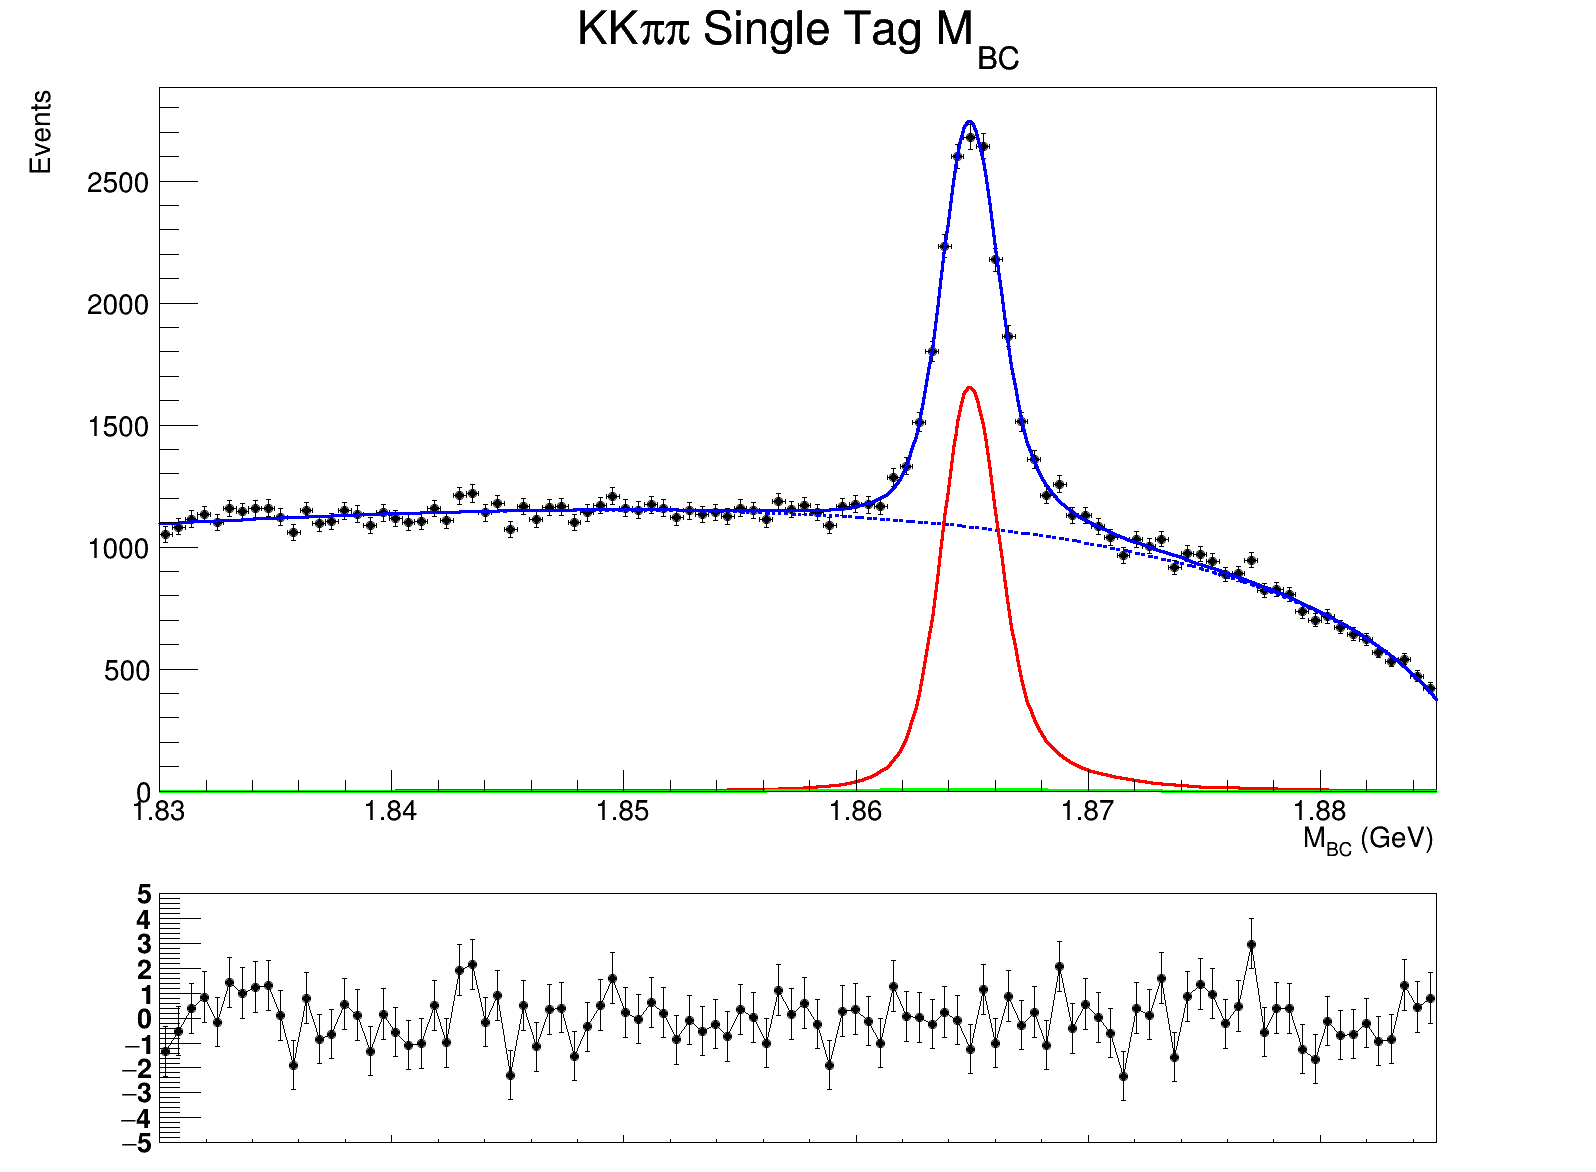
\includegraphics[width=0.6\textwidth]{KKpipiSingleTagMBCPlot.png}
    \caption{$KK\pi\pi$ single tag fit to $m_\text{BC}$, yield: $\SI{10573(174)}{}$}
  \end{figure}
  Question: Should I let the mean of the convolved Gaussian shape float?  \\
  Question: Mass resolution is around $\SI{0.5}{\mega\eV}$, too small?
\end{frame}

\begin{frame}{$K_SKK$ mass veto}
  \begin{figure}
    \centering
    \begin{subfigure}{0.5\textwidth}
      \centering
      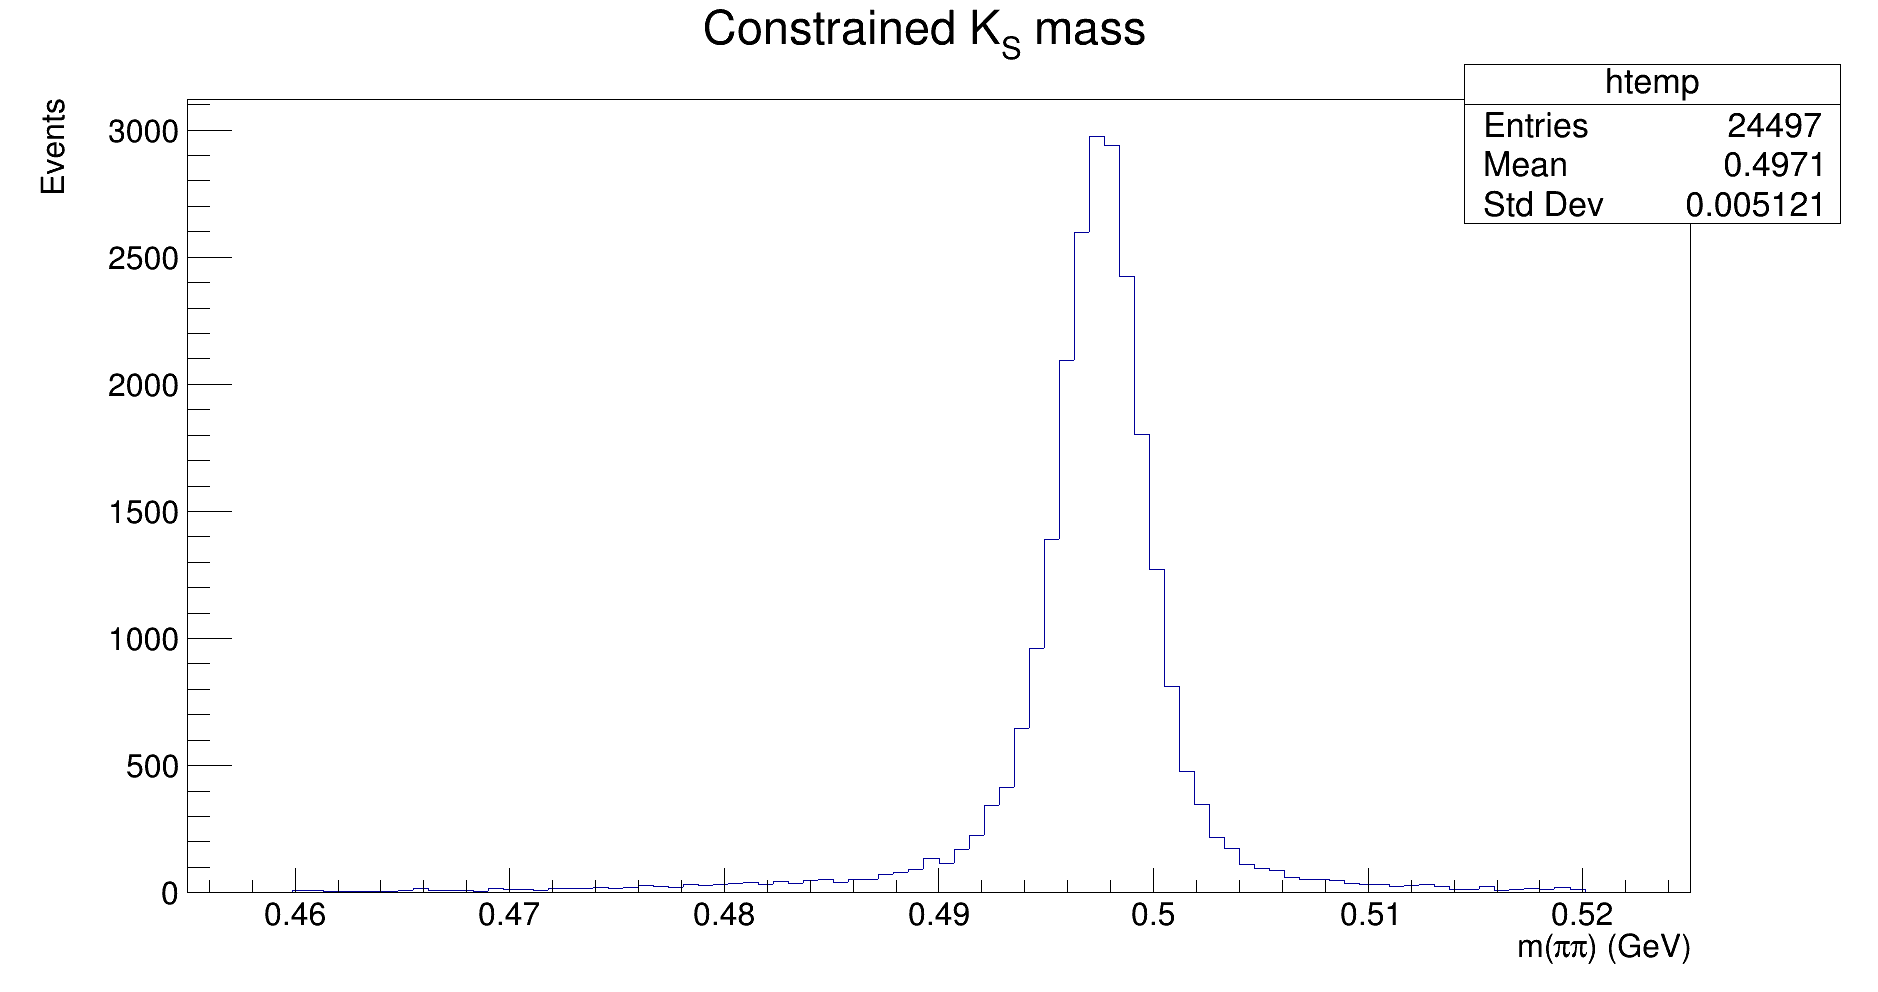
\includegraphics[width=\textwidth]{ConstrainedKSMass.png}
      \caption{$m(\pi\pi)$ constrained}
    \end{subfigure}%
    \begin{subfigure}{0.5\textwidth}
      \centering
      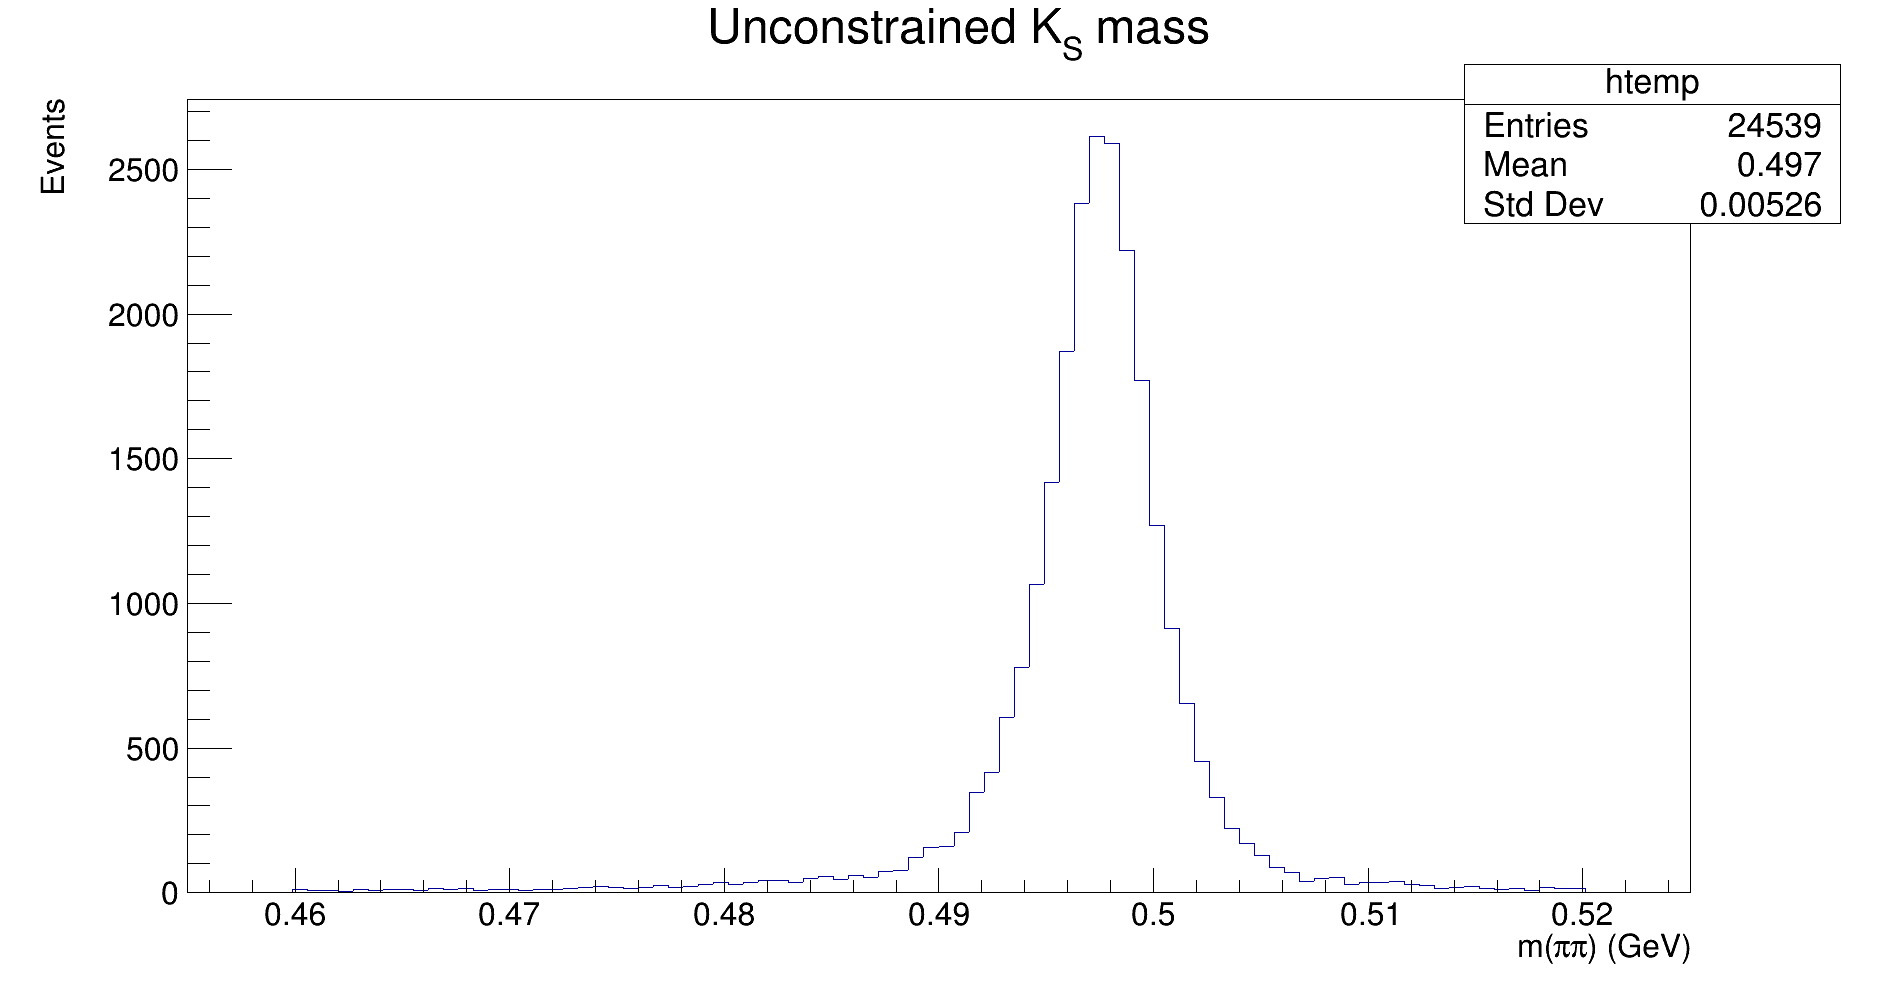
\includegraphics[width=\textwidth]{UnconstrainedKSMass.png}
      \caption{$m(\pi\pi)$ unconstrained}
    \end{subfigure}
  \end{figure}
  Problem: Vertex fit doesn't improve $K_S$ mass resolution...?
\end{frame}

\begin{frame}{$KK$ and $\pi\pi$ single tag yields}
  \begin{figure}
    \centering
    \begin{subfigure}{0.5\textwidth}
      \centering
      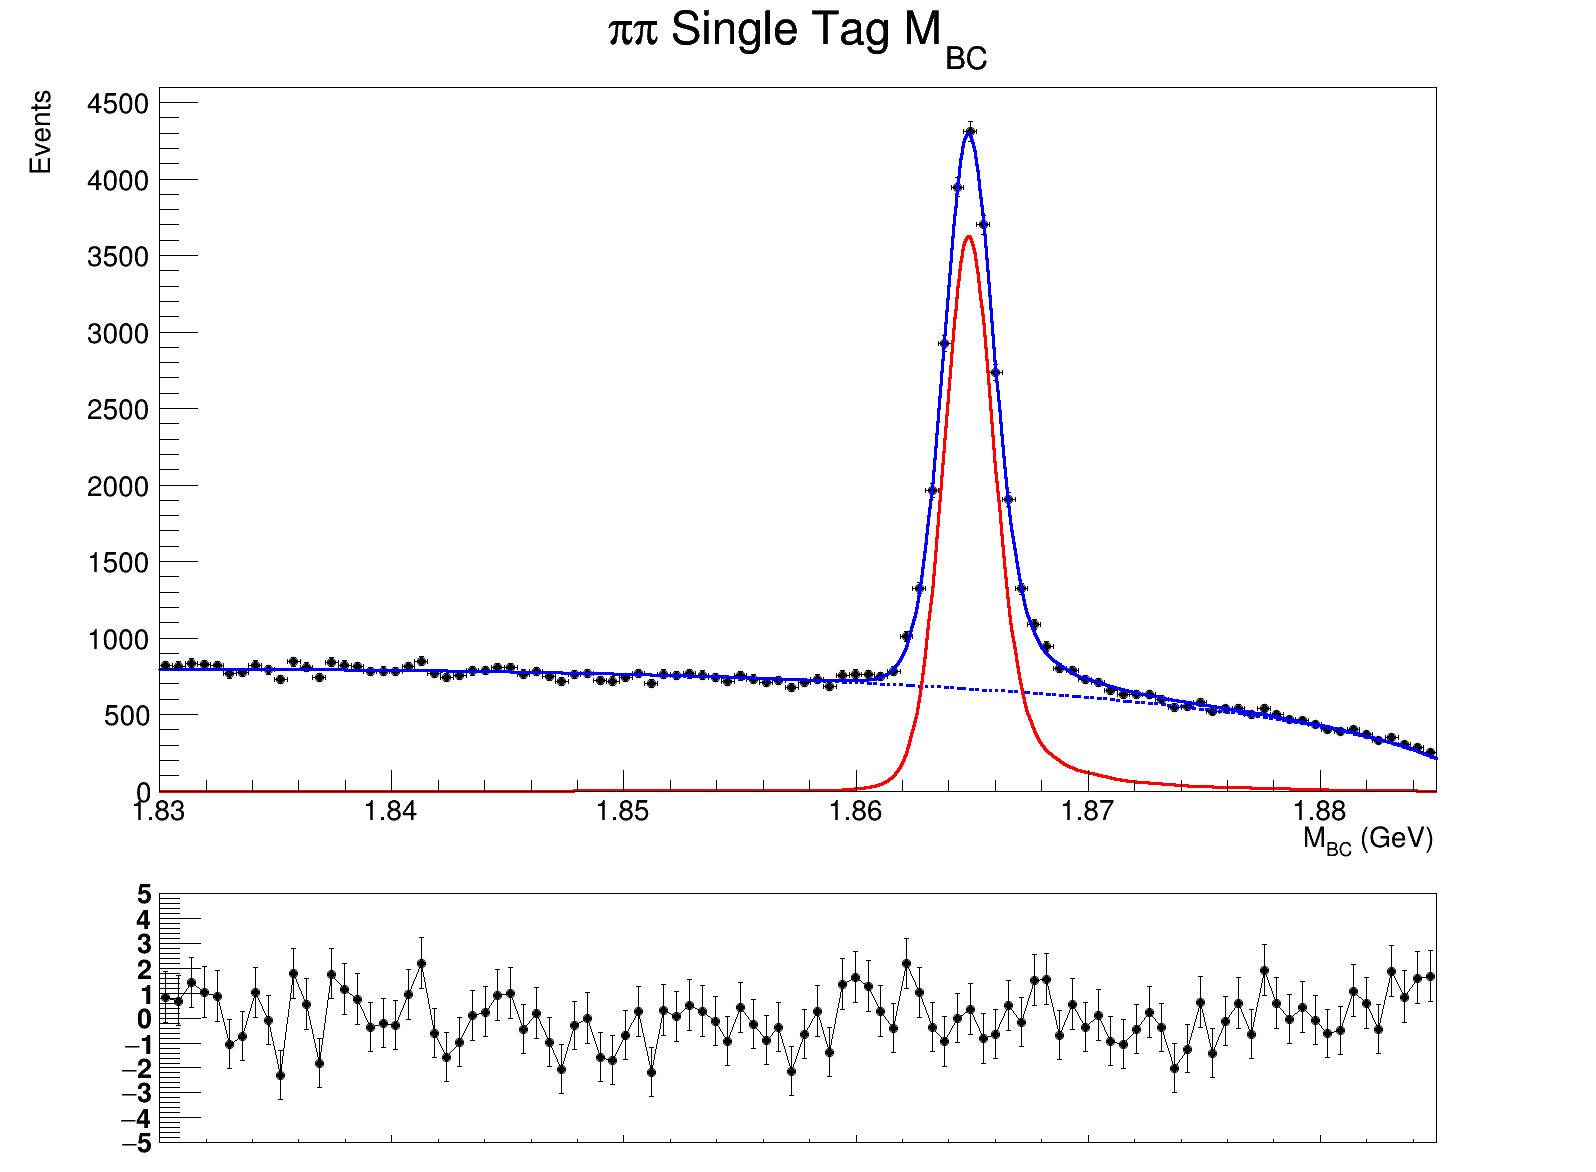
\includegraphics[width=\textwidth]{pipiSingleTagMBCPlot.png}
      \caption{$\pi\pi$ single tag yield: $\SI{19705(177)}{}$}
    \end{subfigure}%
    \begin{subfigure}{0.5\textwidth}
      \centering
      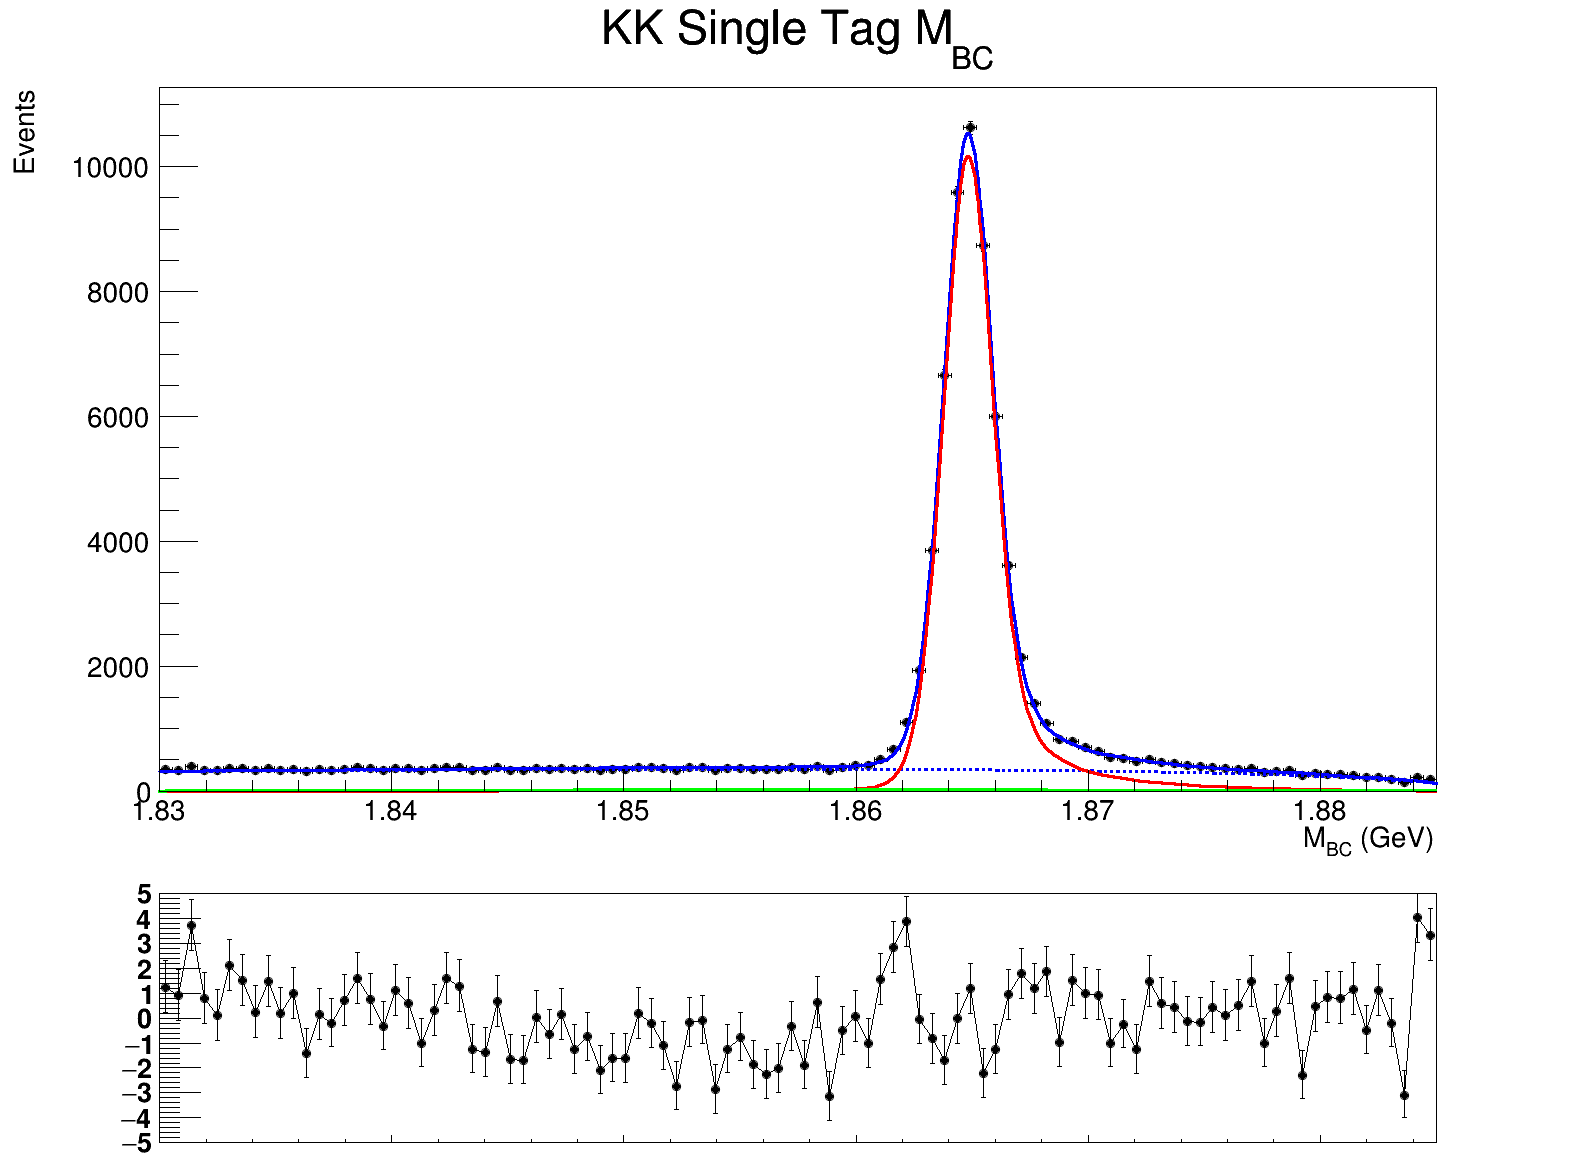
\includegraphics[width=\textwidth]{KKSingleTagMBCPlot.png}
      \caption{$KK$ single tag yield: $\SI{53934(249)}{}$}
    \end{subfigure}
  \end{figure}
  \begin{itemize}
    \item{From $K_SKK$ MEMO: $\SI{19339(163)}{}$ and $\SI{53481(247)}{}$, respectively}
    \item{Lower because $\Delta E$ range was smaller}
  \end{itemize}
\end{frame}

\section{Next steps}
\begin{frame}{Next steps}
  \begin{itemize}
    \setlength\itemsep{2em}
    \item{Code with neutral particle truth matching running}
    \item{Run $m_\text{BC}$ fit for other tag modes}
    \item{Start with DT yields}
  \end{itemize}
\end{frame}

\end{document}
